
% ===============================================

\documentclass[a4paper]{article}
\usepackage[margin=1in]{geometry}
\usepackage{textpos}
\usepackage{enumerate}
\usepackage{amsmath,amsthm,amssymb}
\usepackage[english]{babel}
\usepackage[utf8]{inputenc}
\usepackage{alltt}
\usepackage[]{algorithm2e}
\usepackage{mathtools}
\usepackage{graphicx}

\DeclarePairedDelimiter\ceil{\lceil}{\rceil}
\DeclarePairedDelimiter\floor{\lfloor}{\rfloor}
\begin{document}

% ------------------------------------------ %
%                 START HERE                 %
% ------------------------------------------ %

\title{Variational Canonical Correlation Analysis (VCCA)} % Replace "1" with the appropriate number
\author{Yang Chen} % Replace "Author's Name" with your name
\maketitle
\section{Multi-View Learning task}
In the multi-view representation learning setting, we have multiple views (types of measurements) of the same under- lying signal, and the goal is to learn useful features of each view using complementary information contained in both views. The learned features should uncover the common sources of variation in the views, which can be helpful for exploratory analysis or for downstream tasks.
\section{VCCA}
VCCA models the {\bf joint distribution of two views} with a latent variable model capturing both the shared and private information, where the distributions are parameterized by deep neural networks. VCCA optimizes a {\bf variational lower bound} of the likelihood and allows for straightforward training using small minibatches of training samples.
\section{Latent Variable}
\subsection{}

The probabilistic latent variable model interpretation of linear CCA is shown hare:

\begin{center}
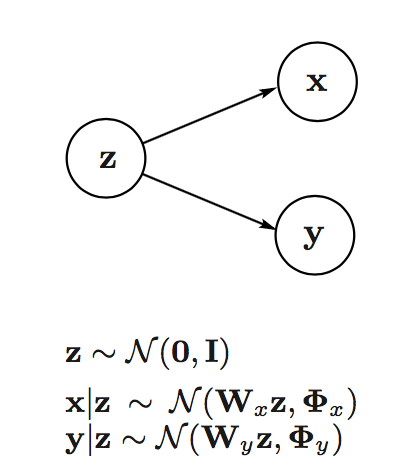
\includegraphics[width=4cm, height=5cm]{lat.png}
\end{center}

Assuming that x and y are linear functions of some random variable z in $R^{d_z}$, where $d_z <= min(d_x,d_y)$. The prior distribution p(z) and conditional distributions $p(x|z)$ and $p(y|z)$ are Gaussian. Jordan showed that $E(z|x)$ lives in the same space as the linear CCA projection for x.

The VCCA model extends the latent variable interpretation of linear CCA to nonlinear observation models parameterized by DNN.
\begin{center}
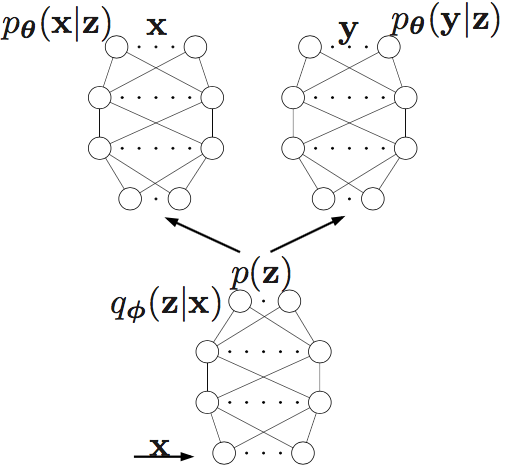
\includegraphics[width=5cm, height=5cm]{vcca.png}

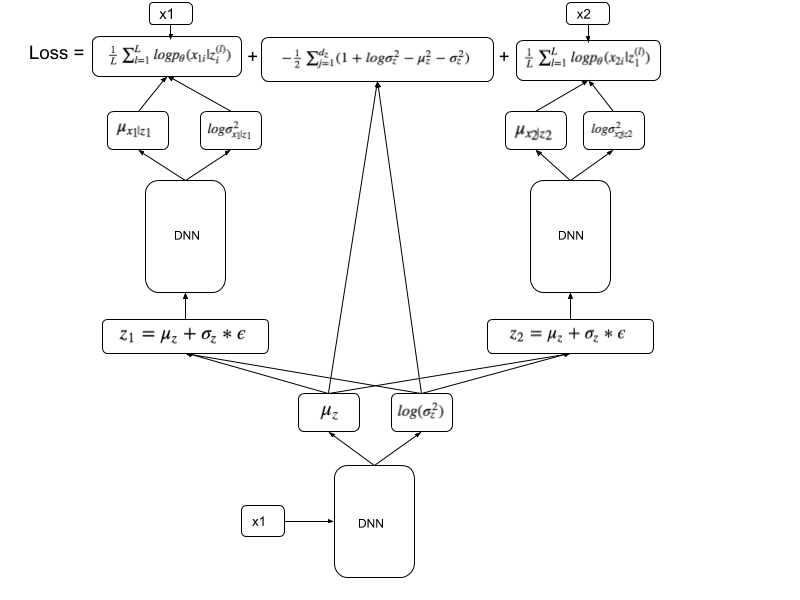
\includegraphics[width=15cm, height=12cm]{vcca_nn.png}
\end{center}
The probabilistic latent variable model of CCA defines the following joint distribution over the random variables (x,y):
    
$p(x,y,z) = p(z)p(x|z)p(y|z)$

$p(x,y)=\int p(x,y,z)dz$

Assumption: x and y are conditionally independent on z.

However, $p_\theta(x,y)$ does not have a closed form, and $p_\theta(z|x)$ is intractable. (Reason: This integral requires exponential time to compute as it needs to be evaluated over all configurations of {\bf latent variables}. So we need to approximate this posterior distribution.)

\section{Objective}
\subsection{Lower Bound}

$logp_\theta(x,y) >= L(x,y;\theta,\Phi) := - D_{KL}(q_\Phi(z|x)||p(z)) + E{q_\Phi(z|x)}[logp_\theta(x|z)+logp_\theta(y|z)]$
\subsection{Derivation of the lower bound}
\begin{align*}
log_{p\theta}(x,y)\\
&= log_{p\theta}(x,y) \int q_\Phi(z|x)dz\\
&= \int log_{p\theta}(x,y) q_\Phi(z|x)dz\\
&= \int q_\Phi(z|x) (log(p(x,y,z)/p(z|x,y)))dz\\
&= \int q_\Phi(z|x) (log(p(x,y,z)/q(z|x)* q(z|x)/p(z|x,y)) dz\\
&= \int q_\Phi(z|x) log\frac{p(x,y,z)}{q(z|x)}dz + \int q_\Phi(z|x) log\frac{q(z|x)}{p(z|x,y)}dz\\
&= E_{q\Phi(z|x)}[log\frac{p_\theta(x,y,z)}{q_\Phi(z|x)}]+ D_{KL}(q_\Phi(z|x)||p_\theta(z|x,y))\\
&>= E_{q\Phi(z|x)}[log\frac{p_\theta(x,y,z)}{q_\Phi(z|x)}] \to (\text{KL is nonnegative})\\
&= L(z,y;\theta,\Phi)
\end{align*}

So 

\begin{align*}
L(x,y;\theta,\Phi)\\
&= \int q_\Phi(z|x)[log \frac{p(z)p(x|z)p(y|z)}{q(z|x)}]dz\\
&= \int q_\Phi(z|x)[log \frac{p(z)}{q(z|x)} + logp(z|x) logp(y|z)]dz\\
&= - D_{KL}(q_\Phi(z|x)||p(z)) + E_{q(z|x)}[log p(x|z) + log p(y|z)]
\end{align*}

\subsection{Compute E part}

$E_{q\Phi(z_i|x_i)}[logp_\theta(x_i|z_i) + logp_\theta(y_i|z_i)]=\frac{1}{L}\sum_{l=1}^L logp_\theta(x_i|z_i^{(l)})+logp_\theta(y_i|z_i^{(l)})$

\subsubsection{Code}
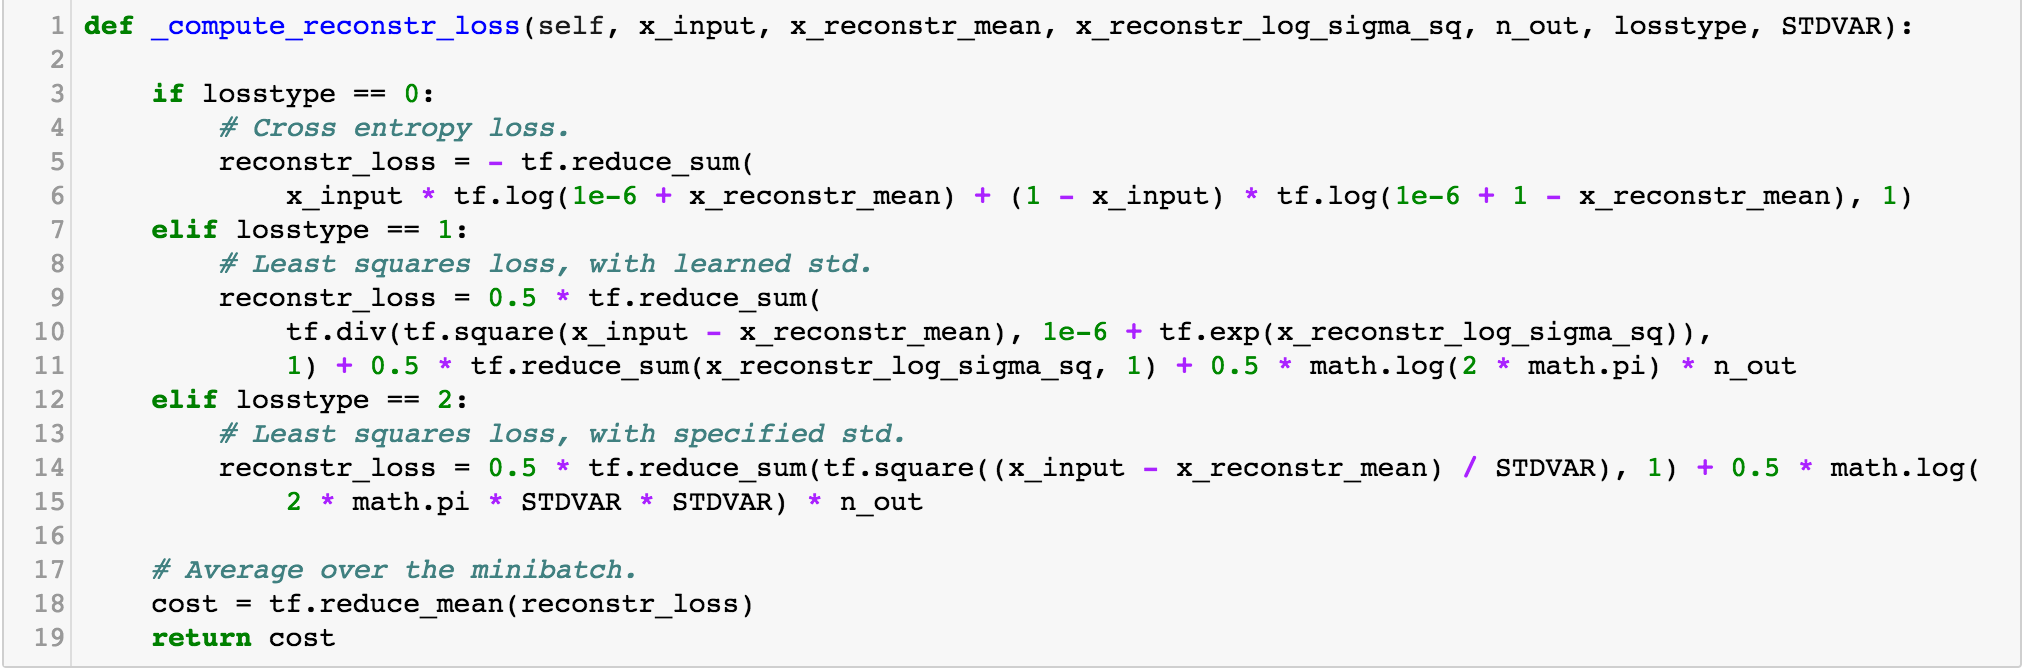
\includegraphics[width=17cm, height=6cm]{loss_code.png}

\subsection{Compute KL divergence}

$D_{KL}(q_\Phi(z_i|x_i)||p(z_i)) = -\frac{1}{2}\sum_{j=1}^{d_z}(1+log\sigma_{ij}^2 - \sigma_{ij}^2 - \mu_{ij}^2)$


\subsubsection{Derivation of KL divergence}
Assumption random variable x1,x2 is Gaussian distribution. $x1\to N_1(\mu_1,\sigma_1^2), x2\to N_2(\mu_2,\sigma_2^2)$. 

$N(\mu,\sigma^2) = \frac{1}{\sqrt{2\pi\sigma^2}}e^{\frac{(x-\mu)^2}{2\sigma^2}}$

\begin{align*}
&\int p_1(x)log\frac{p_1(x)}{p_2(x)} dx\\
&= \int p_1(x) (logp_1(x) - logp_2(x))dx\\
&= \int p_1(x) (log \frac{1}{\sqrt{2\pi\sigma_1^2}}e^{\frac{(x-\mu_1)^2}{2\sigma_1^2}} -log \frac{1}{\sqrt{2\pi\sigma_2^2}}e^{\frac{(x-\mu_2)^2}{2\sigma_2^2}})dx\\
&= \int p_1(x) (-1/2 log2\pi - log\sigma_1 - \frac{(x-\mu_1)^2}{2\sigma_1^2} + 1/2 log2\pi + log \sigma_2 + \frac{(x-\mu_2)^2}{2\sigma_2^2})dx\\
&= \int p_1(x)(log\frac{\sigma_1}{\sigma_2} + [\frac{(x-\mu_1)^2}{2\sigma_1^2} - \frac{(x-\mu_2)^2}{2\sigma_2^2}]) dx\\
&= \int (log\frac{\sigma_2}{\sigma_1}p_1(x)dx + \int \frac{(x-\mu_1)^2}{2\sigma_1^2} p_1(x)dx - \int \frac{(x-\mu_2)^2}{2\sigma_2^2} p_1(x) dx\\
&= log\frac{\sigma_1}{\sigma_2} + \frac{1}{2\sigma_2^2}\int (x-\mu_2)^2p_1(x)dx - \frac{1}{2\sigma_1^2}\int (x-\mu_1)^2 p_1(x)dx\\
&= log\frac{\sigma_1}{\sigma_2} + \frac{1}{2\sigma_2^2}\int (x-\mu_2)^2p_1(x)dx - \frac{1}{2} \to (\int (x-\mu_1)^2 p_1(x)dx=\sigma_1^2)\\
&= log\frac{\sigma_1}{\sigma_2} + \frac{1}{2\sigma_2^2}\int (x-\mu_1+\mu_1-\mu_2)^2p_1(x)dx - \frac{1}{2}\\
&= log\frac{\sigma_1}{\sigma_2} + \frac{1}{2\sigma_2^2}[\int (x-\mu_1)^2p_1(x)dx + \int (\mu_1-\mu_2)^2p_1(x)dx + 2\int(x-\mu_1)(\mu_1-\mu_2)p_1(x)dx] - \frac{1}{2}\\
&=log\frac{\sigma_1}{\sigma_2} + \frac{1}{2\sigma_2^2}[\int (x-\mu_1)^2p_1(x)dx +(\mu_1-\mu_2)^2] - \frac{1}{2}\\
&\to (2\int(x-\mu_1)(\mu_1-\mu_2)p_1(x)dx = (\mu_1-\mu_2)\int (x-\mu_1)p_1(x)dx \\
&= (\mu_1-\mu_2)[\int xp_1(x)dx - \int \mu_1p_1(x)dx] = (\mu_1-mu_2)[\mu_1-\mu_1]=0\\
&= log\frac{\sigma_2}{\sigma_1}+\frac{\sigma_1^2+(\mu_1-\mu_2)^2}{2\sigma_2^2} - \frac{1}{2})\\
&\text{Let }\mu_2 = 0, \sigma_2^2 = 1\\
&= -log \sigma_1 + \frac{\sigma_1^2+\mu_1^2}{2}-\frac{1}{2}\\
&= -\frac{1}{2}(1 + 2log \sigma_1 - \sigma_1^2-\mu_1^2)\\
&= -\frac{1}{2}(1 + log \sigma_1^2 - \sigma_1^2-\mu_1^2)
\end{align*}

\subsubsection{Code}
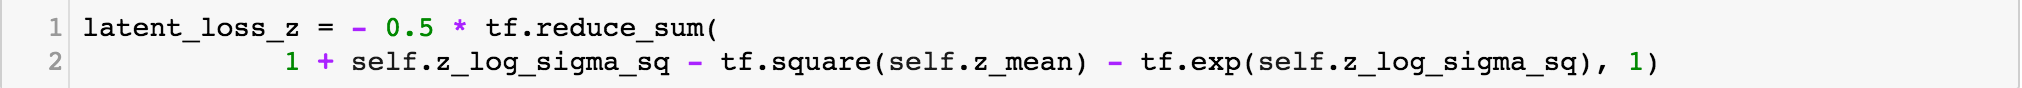
\includegraphics[width=17cm, height=0.8cm]{kl_code.png}
\section{Reparameterization trick}

Intuitively, in its original form, VAEs sample from a random node z which is approximated by the parametric model $q(z | \Phi,x)$ of the true posterior. Backprop cannot flow through a random node.

Introducing a new parameter $\epsilon$ allows us to reparameterize z in a way that allows backprop to flow through the deterministic nodes.
\begin{center}
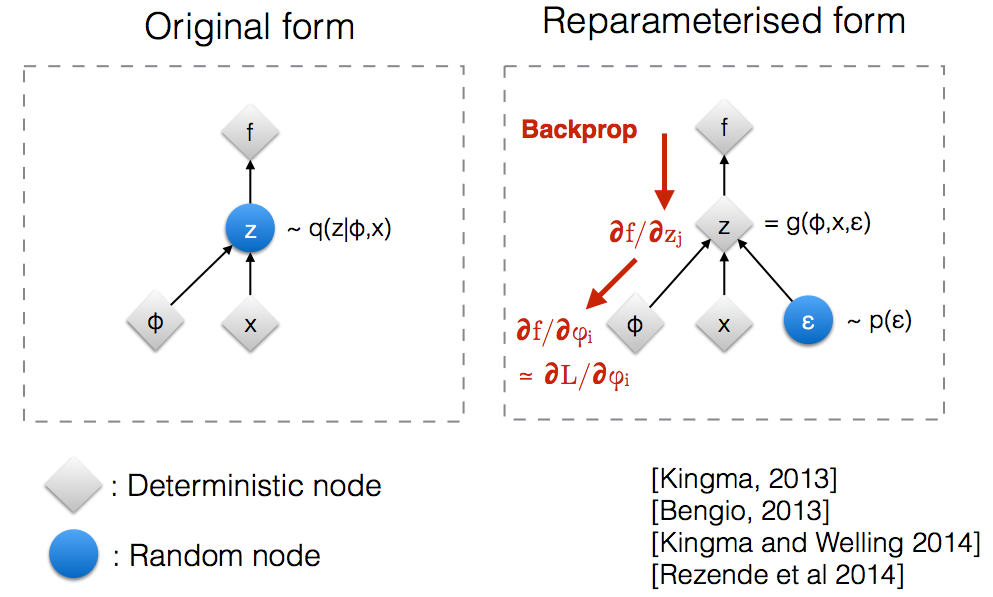
\includegraphics[width=10cm, height=6cm]{repara.png}
\end{center}
\subsection{Code}
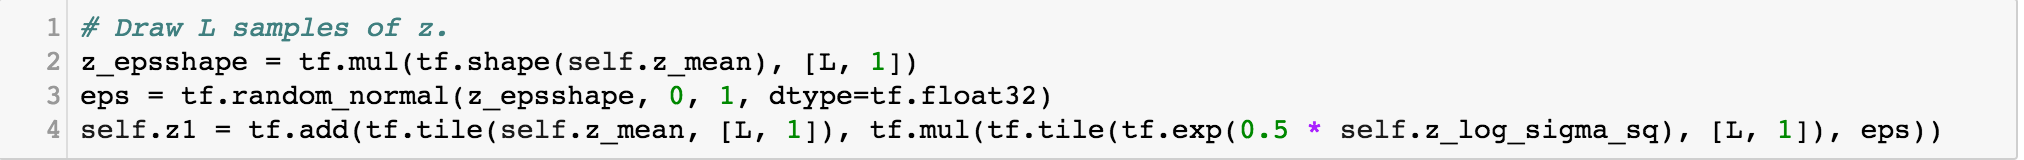
\includegraphics[width=17cm, height=1.5cm]{repa_code.png}
\section{Deep Neural Network}

We consider non-linear observation models $p_\theta(x|z;\theta_x), p_\theta(y|z;\theta_y)$, parameterized by $\theta_x$ and $\theta_y$, which can be the collections of weights of DNNs. We also approximate $p_\theta(z|x)$ with the conditional density $q_\Phi(z|x;\Phi_z)$, where $\Phi_z$ is the collection of parameters of another DNN.

\subsection{Code}

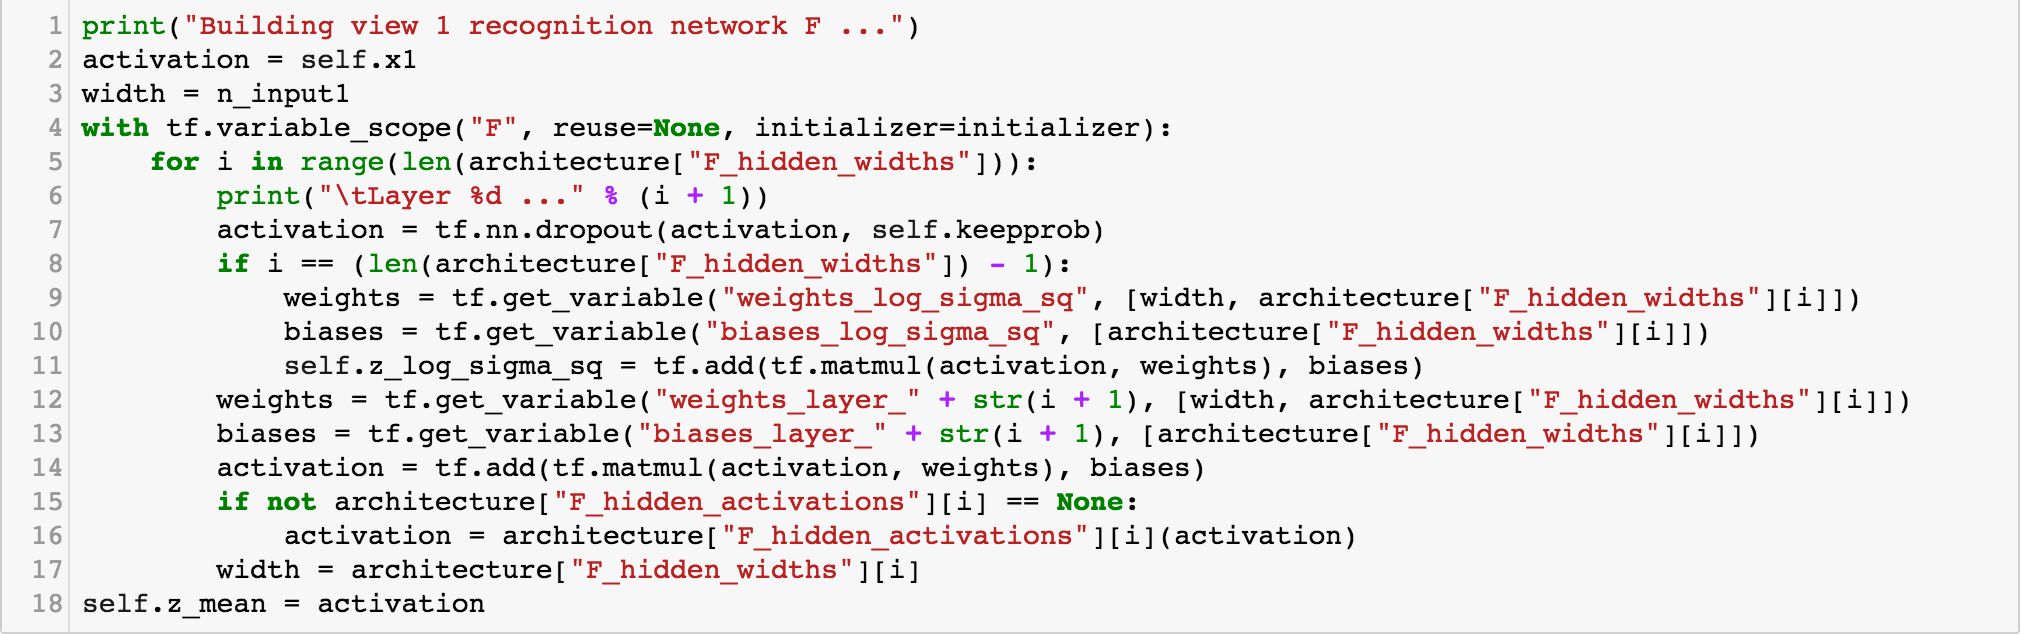
\includegraphics[width=17cm, height=6cm]{dnn_code.png}

\section{Private information}
There might be large variations in the input space that can not be explained by the common variables. It may then be beneficial to explicitly model the private variables within each view.
\begin{center}
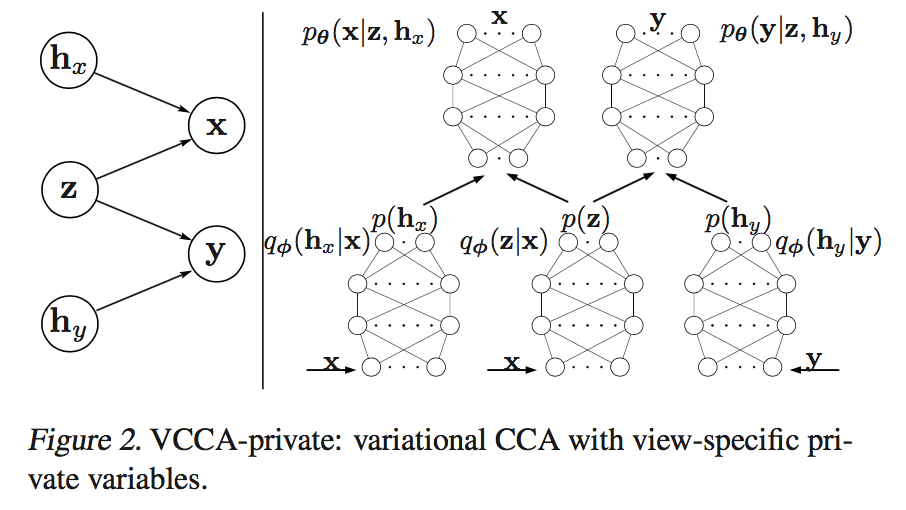
\includegraphics[width=10cm, height=6cm]{vcca-p.png}
\end{center}

\section{VCCA-p for acoustic feature learning}

Apply VCCA and VCCA-p on the X-ray Microbeam Database.

acoustic:
\begin{center}
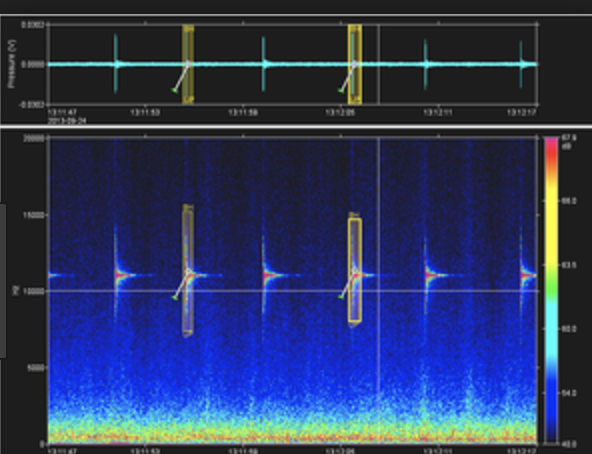
\includegraphics[width=10cm, height=6cm]{acous.png}
\end{center}

articulatory:
\begin{center}
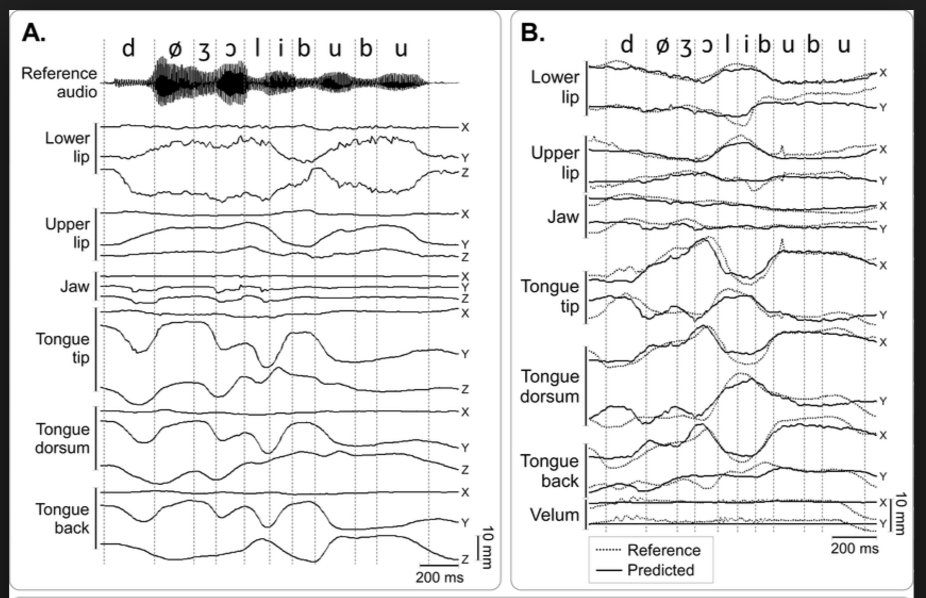
\includegraphics[width=10cm, height=6cm]{art.png}
\end{center}

\subsection{Generative adversrial training}

We extend VCCA/VCCAP with generative adversarial training by viewing the basic VCCA/VCCAP model as a pair of generators, and adding two discriminators D1 and D2, one for each view, which try to distinguish the generated samples from training set unput samples.

\begin{center}
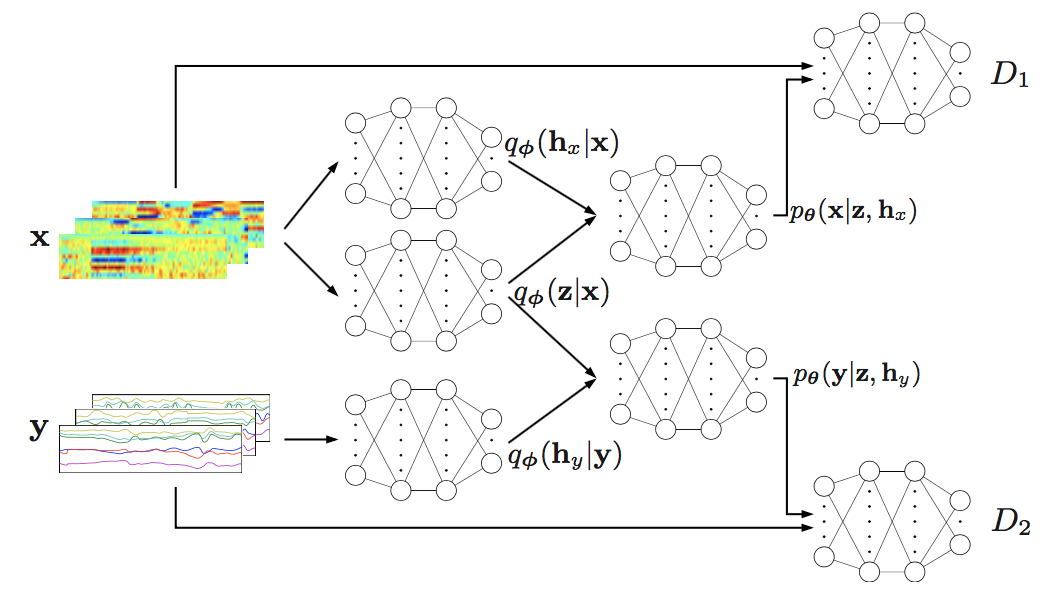
\includegraphics[width=10cm, height=6cm]{vccapg.png}
\end{center}

D1 optimizes:

$max_{D1} logD_1(x_i)+log(1-D1(x_i'))$, 

where x is the original input of the first view and x' is the corresponding reconstruction.

The generator optimize:

$max_{\theta,\Phi} L_{private}(x_i,y_i;\theta,\Phi) + \lambda_1log(D1(x_i'))+\lambda_2log(D2(y_i'))$


%%%%%%%%%%%%%%%%%%%%%%%%%%%%%%%%%%%%%%%%%%%%%%%
\section{Related work}
\subsection{Canonical Correlation Analysis}

Let $X^{(1)}$ be a p by 1 vector and $X^{(2)}$ be a q by 1 vector, $p<=q$

Let $E(X^{1}) = \mu^1_{(p*1)}; Cov(X^1) = \Sigma_{11(p*p)}$
$E(X^{2}) = \mu^2_{(q*1)}; Cov(X^2) = \Sigma_{22(q*q)}$

and

$Cov(X^1,X^2) = \Sigma_{12} = \Sigma_{21}^T$,
$E[[X^1 - \mu^1][X^2 - \mu^2]^T]$ is a p by q matrix.

So:

\begin{center}
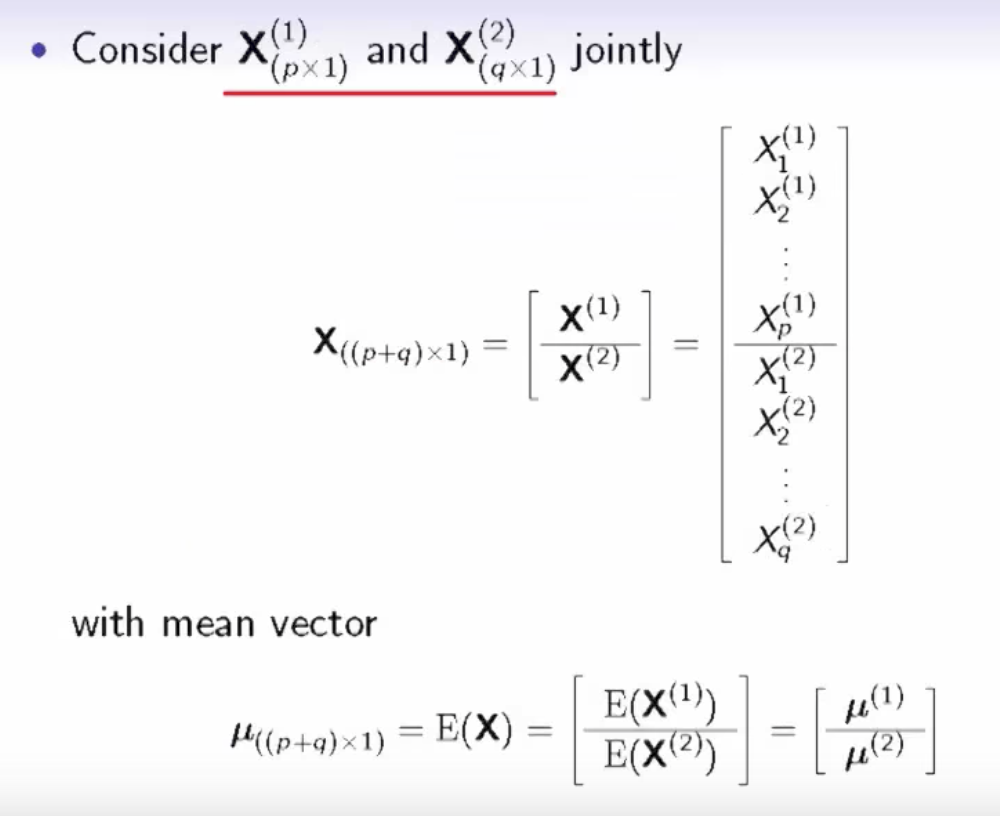
\includegraphics[width=10cm, height=7cm]{ex.png}
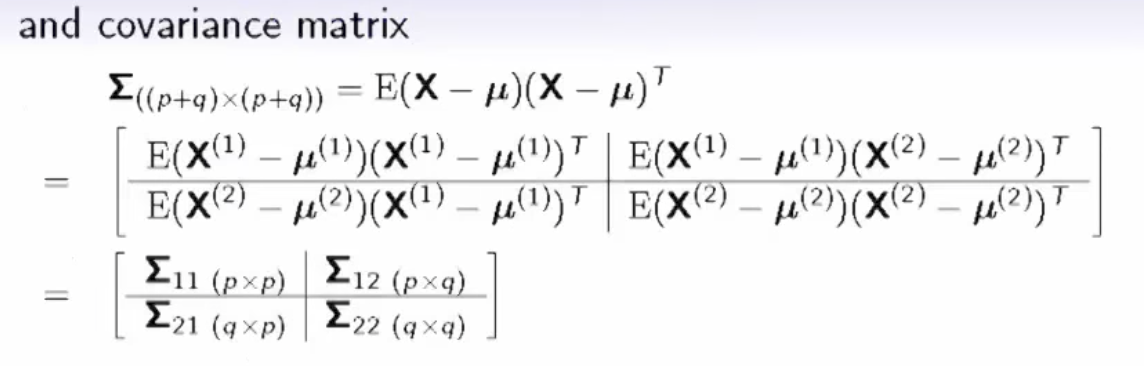
\includegraphics[width=10cm, height=3cm]{cov.png}
\end{center}

Set linear combinations:

$U=a^T X^1, V = b^TX^2$

We can obtain:
\begin{align*}
Var(U) &= a^T Cov(X^1)a = a^T \Sigma_{11}a\\
Var(V) &= b^T Cov(X^2)b = b^T \Sigma_{22}b\\
Cov(U,V) &= a^T Cov(X^1,X^2)b = a^T \Sigma_{12}b
\end{align*}

We seek coefficient vectors a and b such that

$Corr(U,V) = \frac{a^T\Sigma_{12}b}{\sqrt{a^T\Sigma_{11}a}\sqrt{b^T\Sigma_{22}b}}$

is as large as possible.

Variance of U and V = 1.


Define:

kth canonical variate pair = the pair of linear combination $U_k$ and $V_k$ having
unit variances, which maximize the correlation among all {\bf choices uncorrelated with
the previous k - 1 canonical variate pairs.}
Note: uncorrelated does not equal to independent!
\begin{center}
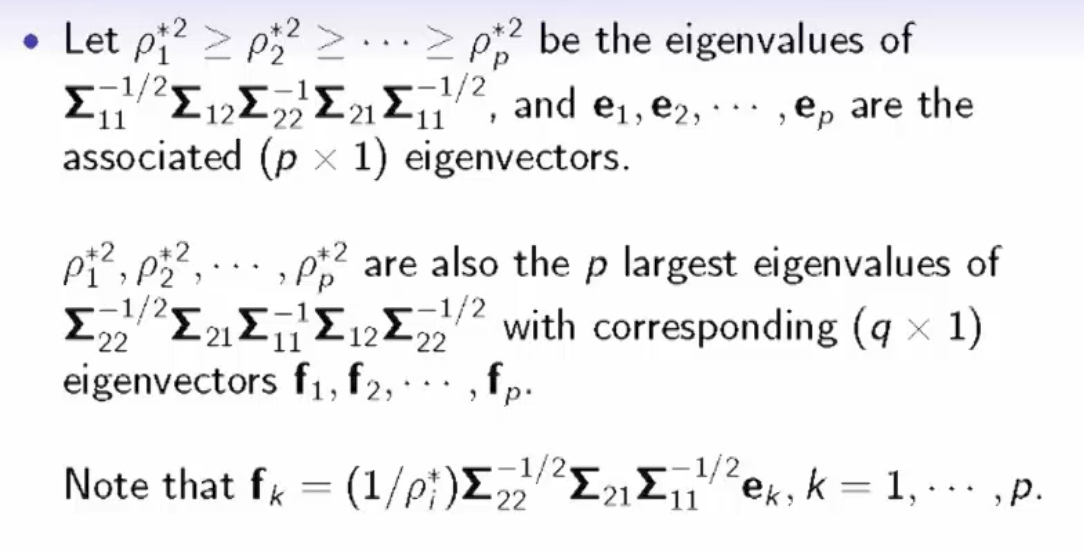
\includegraphics[width=10cm, height=6cm]{eig.png}
\end{center}

Result:

$Max_{a,b} Corr(U,V) = \rho^*_1$

attained by the linear combinations

$U_1 = e_1^T \Sigma_{11}^{-1/2}X^1$ and $V_1 = f_1^T \Sigma_{22}^{-1/2} X^2$

The canonical variates have the properties
$Var(U_k) = Var(V_k) = 1$

$Cov(U_k,U_l) = Cov(V_k,V_l) = Cov(U_k,V_l) = 0$ when $k != l$

\subsubsection{Canonical variates from standardized variables}

$Z^1 = [Z_1^1,Z_2^1,...,Z_p^1]^T$ and

$Z^2 = [Z_1^2, Z_2^2,...,Z_q^2]^T$

Here, $Cov(Z^1) = \rho_{11}, Cov(Z^2) = \rho_{22}$, and

$Cov(Z^1,Z^2) = \rho_{12}=\rho_{21}^T$.

Then use
$\rho_{11}^{-1/2}\rho_{12}\rho_{22}^{-1}\rho_{21}\rho_{11}^{-1/2}$
find eigenvalues and eigenvectors. Eigenvalues are the same as before but the eigenvectors are different.

\begin{center}
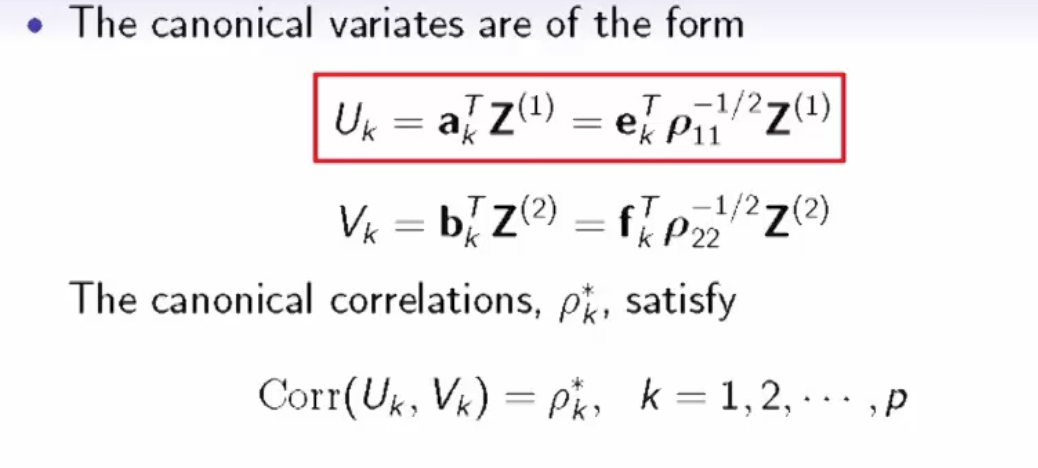
\includegraphics[width=10cm, height=5cm]{z.png}
\end{center}

$a^T_k(X^1-\mu^1) = a_k^T V_{11}^{1/2}Z^1$
where $V_{11}$ is the diagonal matrix with ith element $Var(X_i^1)$.

\subsubsection{Interpretation}

Look at the linear combinatin: $U_1 = a_{11}X_1^1 + a_{12}X_2^1+..$
1. $Corr(U_1, X_1^1)$... Here the correlation != the coefficient

Note p.18:
$\rho_{U,X^1} = Corr(U,X^1) = I^{-1/2}Cov(U,X^1)V_{11}^{-1/2} = A\Sigma_{11}V_{11}^{-1/2}$

\subsubsection{Code}
\begin{verbatim}
def CCA_Mardia(H1, H2, dim):
    # H1 and H2 are NxD matrices containing samples rowwise.
    # dim is the desired dimensionality of CCA space.
    
    d1 = H1.shape[0]
    d2 = H2.shape[0]
    N = H1.shape[1]
    
    # Remove mean
    m1 = np.mean(H1, axis=1)
    m2 = np.mean(H2, axis=1)
    H1 = H1 - np.reshape(m1,(d1,1))
    H2 = H2 - np.reshape(m2,(d2,1))
    
    S11 = (dot(H1,np.transpose(H1)))/(N-1)
    S22 = (dot(H2,np.transpose(H2)))/(N-1)
    S12 = (dot(H2,np.transpose(H1)))/(N-1)

    D1,V1 = la.eig(S11)
    D2,V2 = la.eig(S22)

    K11 = dot(dot(V1,np.diag(1/np.sqrt(D1))),np.transpose(V1))
    K22 = dot(dot(V2,np.diag(1/np.sqrt(D2))),np.transpose(V2))

    T = dot(dot(K22,S12),K11)
    U,D,V = np.linalg.svd(T)
    D = np.diag(D)
    A = dot(K11,np.transpose(V[0:dim,:]))
    B = dot(K22,np.transpose(U[0:dim,:]))
    D = D[0:dim]
    return A,B,D
\end{verbatim}

\subsection{Kernel Canonical Correlation Analysis}
Kernel CCA offers an alternative solution by first projecting the data into a higher-dimensional feature space.

$\Phi: x = (x_1,...,x_m) \to \Phi(x) = (\Phi_1(x),...,\Phi_N(x)) (m<N)$

Kernel is known as the kernel trick. A kernel is a function K, such that for all x,z in X, 

$K(x,z) = <\Phi(x)*\Phi(z)>$,

where $\Phi$ is a mapping from X to a feature space F.

We can rewrite the covariance matrix C using the data matrices X and Y, which have the sample vector as rows and are therefore of size m by N; we obtain

$C_{xx} = X'X, C_{xy}=X'Y$.

Then $w_{x(N*1)} = X_{N*m}'\alpha_{m*1}, w_{y(N*1)}=Y_{N*m}'\beta_{m*1}$.

So $\rho = max_{\alpha,\beta} \frac{\alpha'XX'YY'\beta}{\sqrt{\alpha'XX'XX'\alpha * \beta'YY'YY'\beta}}$

Let $K_x = XX', K_y = YY'$ be the kernel matrices, we have

$\rho = max_{\alpha,\beta} \frac{\alpha'K_xK_y\beta}{\sqrt{\alpha'K_x^2\alpha \beta'K_y^2\beta}}$

So it is equivalent to maxmizing the numerator subject to denominator = 1.

\subsubsection{Regularization}
It combine the PLS term with the KCCA term in the denominator, obtaining:

$\rho = max_{\alpha,\beta} \frac{\alpha'K_xK_y\beta}{\sqrt{(\alpha'K_x^2\alpha+k||w_x||^2)(\beta'K^2_y\beta+k||w_y||^2)}}
=max_{\alpha,\beta} \frac{\alpha'K_xK_y\beta}{\sqrt{(\alpha'K_x^2\alpha+k\alpha'K_x\alpha)(\beta'K^2_y\beta+k\beta'K_y\beta)}}$

obtain a standard eigenproblem of the form $Ax=\lambda x$.

\subsubsection{Partial Gram-Schmidt Orthogonalization}

Use PGSO as matrix decomposition approach.

problem:
KCCA involves and N by N eigenvalue problem and so is challenging in both memory and time (O(N3)). Several approximation methods have been proposed.

\subsection{Deep Canonical Correlation Analysis (DCCA)}
Deep CCA computes representations of the two views by passing them
through multiple stacked layers of nonlinear transformation.

\begin{center}
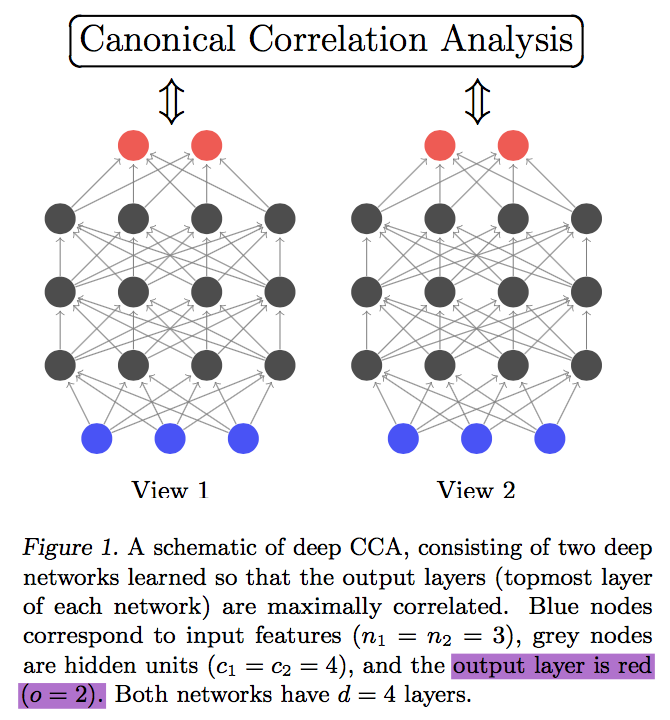
\includegraphics[width=6cm, height=6cm]{dnet.png}
\end{center}


The goal is to jointly learn parameters for both views $W_l^v. b_l^v$ such that $corr(f_1(X_1),f_2(X_2))$ is as high as possible.

Note: o is the number of output. This corresponds to the number of component in CCA.

$(\theta_1^*,\theta_2^*) = argmax_{\theta_1,\theta_2} corr(f_1(X_1),f_2(X_2))$

To find $(\theta_1^*,\theta_2^*)$, we follow the gradient of the correlation objective as estimated on the training data.

k = o, so the output is the number of top k components of H1 and H2.


\subsubsection{Use L-BFGS second-order optimization method}

\subsubsection{Non-saturating nonlinearity}

Best results are obtained by using $g(y)=g^3/3+y, s(x)=g^{-1}(x)$

1. s is not bounded, and its derivative falls off much more gradually with x.

2. it derivative is a simple function of its value

\subsubsection{Code}
Python code:https://github.com/VahidooX/DeepCCA

Let's look at the loss function: $y_{true}$ is ignored, that is the
reason it return {\bf -corr. We want to maximize the correlation = minimize the loss(-corr).}

\subsubsection{Objective function}
\begin{verbatim}
def cca_loss(outdim_size, use_all_singular_values):
    """
    The main loss function (inner_cca_objective) is wrapped in this function due to
    the constraints imposed by Keras on objective functions
    """
    def inner_cca_objective(y_true, y_pred):
        """
        It is the loss function of CCA as introduced in the original paper. There can be other formulations.
        It is implemented by Theano tensor operations, and does not work on Tensorflow backend
        y_true is just ignored
        """

        r1 = 1e-4
        r2 = 1e-4
        eps = 1e-12
        o1 = o2 = y_pred.shape[1]//2

        # unpack (separate) the output of networks for view 1 and view 2
        H1 = y_pred[:, 0:o1].T
        H2 = y_pred[:, o1:o1+o2].T

        m = H1.shape[1]

        H1bar = H1 - (1.0 / m) * T.dot(H1, T.ones([m, m]))
        H2bar = H2 - (1.0 / m) * T.dot(H2, T.ones([m, m]))

        SigmaHat12 = (1.0 / (m - 1)) * T.dot(H1bar, H2bar.T)
        SigmaHat11 = (1.0 / (m - 1)) * T.dot(H1bar, H1bar.T) + r1 * T.eye(o1)
        SigmaHat22 = (1.0 / (m - 1)) * T.dot(H2bar, H2bar.T) + r2 * T.eye(o2)

        # Calculating the root inverse of covariance matrices by using eigen decomposition
        [D1, V1] = T.nlinalg.eigh(SigmaHat11)
        [D2, V2] = T.nlinalg.eigh(SigmaHat22)

        # Added to increase stability
        posInd1 = T.gt(D1, eps).nonzero()[0]
        D1 = D1[posInd1]
        V1 = V1[:, posInd1]
        posInd2 = T.gt(D2, eps).nonzero()[0]
        D2 = D2[posInd2]
        V2 = V2[:, posInd2]

        SigmaHat11RootInv = T.dot(T.dot(V1, T.nlinalg.diag(D1 ** -0.5)), V1.T)
        SigmaHat22RootInv = T.dot(T.dot(V2, T.nlinalg.diag(D2 ** -0.5)), V2.T)

        Tval = T.dot(T.dot(SigmaHat11RootInv, SigmaHat12), SigmaHat22RootInv)

        if use_all_singular_values:
            # all singular values are used to calculate the correlation
            corr = T.sqrt(T.nlinalg.trace(T.dot(Tval.T, Tval)))
        else:
            # just the top outdim_size singular values are used
            [U, V] = T.nlinalg.eigh(T.dot(Tval.T, Tval))
            U = U[T.gt(U, eps).nonzero()[0]]
            U = U.sort()
            corr = T.sum(T.sqrt(U[0:outdim_size]))

        return -corr

    return inner_cca_objective
\end{verbatim}
\subsubsection{SVM classifier}
\begin{verbatim}
def svm_classify(data, C):
    """
    trains a linear SVM on the data
    input C specifies the penalty factor of SVM
    """
    train_data, _, train_label = data[0]
    valid_data, _, valid_label = data[1]
    test_data, _, test_label = data[2]

    print('training SVM...')
    clf = svm.LinearSVC(C=C, dual=False)
    clf.fit(train_data, train_label.ravel())

    p = clf.predict(test_data)
    test_acc = accuracy_score(test_label, p)
    p = clf.predict(valid_data)
    valid_acc = accuracy_score(valid_label, p)

    return [test_acc, valid_acc]
\end{verbatim}

\subsection{Deep Canonically correlated autoencoders (DCCAE)}

multiple views of data at training time while only one view is available at test time:

1. audio + video

2. audio + atriculation

3. images + text

4. parallel text in two languages

5. words + context

6. document txt + text of inbound hyperlinks

This presents an opportunity to learn better representations by analyzing multiple views simultaneously.

Typical approach: learning a feature transformation of the primary view that captures useful information from the second view using a paired two-view training set.

1. auotoencoders: the objective is to learn a compact representation that best reconstructs the inputs

2. CCA: learns features in two views that are maximally correlated

\subsubsection{Split autoencoders (SplitAE)}

extract shared reprensentations by reconstructing both views from the one view that is available at test time. feature extraction network f is shared while the reconstruction network p and q are separate for each view.

object is the sum of reconstruction errors for the two views:
$min_{w_f,w_p,w_q} 1/N \sum_{i=1}^N (||x_i - p(f(x_i))||^2 + ||y_i-q(g(x_i))||^2)$

\begin{center}
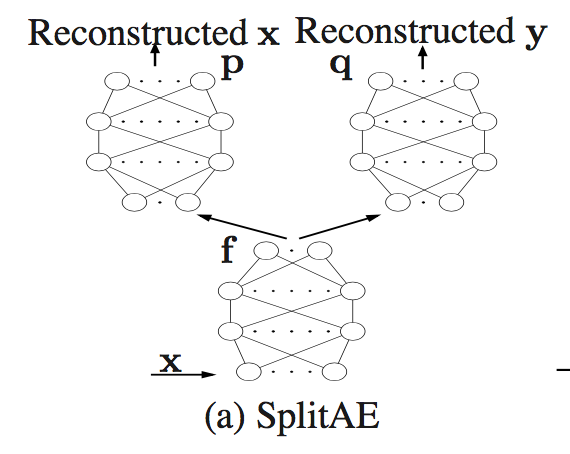
\includegraphics[width=6cm, height=6cm]{splitae.png}
\end{center}

\subsubsection{DCCAE}

object:
$min_{w_f,w_g,w_p,w_q,U,V} -1/N tr(U^Tf(X)g(Y)^TV) + \lambda/N \sum_{i=1}^N (||x_i - p(f(x_i))||^2 + ||y_i-q(g(x_i))||^2)$

\begin{center}
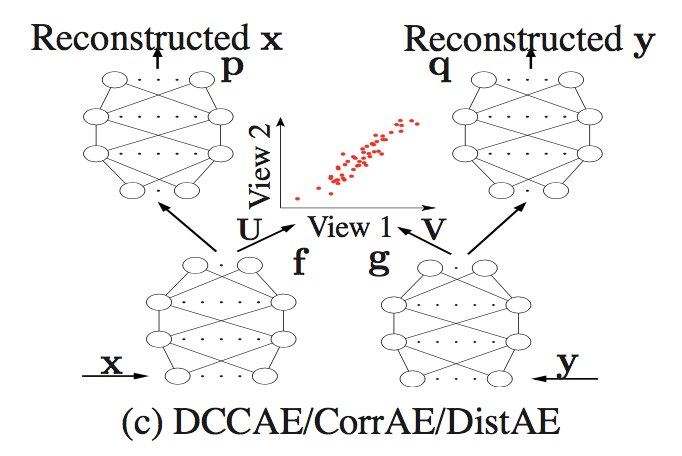
\includegraphics[width=7cm, height=6cm]{dccae.png}
\end{center}

CCA maximizes the mutual information between the projected views for certain distributions;

Autoencoder minimizes reconstruction error amounts to maximizing a lower bound on the mutual information between inputs and learned features.

\subsubsection{Minimum-distance autoencoders (DistAE)}

The CCA objective can be seen as minimizing the distance between the learned projections of the two views, while satisfying the whitening constraints for the projections. The constraints complicate the optimization of CCA-based objectives.

object:
$min_{w_f,w_g,w_p,w_q,U,V} -1/N \sum_{i=1}^N \frac{||f(x_i)-g(y_i)||^2}{||f(x_i)||^2+||g(y_i)||^2}+ \lambda/N \sum_{i=1}^N (||x_i - p(f(x_i))||^2 + ||y_i-q(g(x_i))||^2)$

\subsection{Variational Autoencoder (VAE)}
We simply tell our network what we want this distribution to look like.

Usually, we will constrain the network to produce latent vectors having entries that follow the unit normal distribution. Then, when trying to generate data, we can simply sample some values from this distribution, feed them to the decoder, and the decoder will return us completely new objects that appear just like the objects our network has been trained with.

the encoder is supposed to create objects following a Gaussian Distribution:
1. A vector of means
2. A vector of standard deviations

\subsubsection{Encoder}

The returned values that will be fed to the decoder are the z-values.
\begin{verbatim}
def encoder(X_in, keep_prob):
    activation = lrelu
    with tf.variable_scope("encoder", reuse=None):
        X = tf.reshape(X_in, shape=[-1, 28, 28, 1])
        x = tf.layers.conv2d(X, filters=64, kernel_size=4, strides=2, 
        padding='same', activation=activation)
        x = tf.nn.dropout(x, keep_prob)
        x = tf.layers.conv2d(x, filters=64, kernel_size=4, strides=2, 
        padding='same', activation=activation)
        x = tf.nn.dropout(x, keep_prob)
        x = tf.layers.conv2d(x, filters=64, kernel_size=4, strides=1,
         padding='same', activation=activation)
        x = tf.nn.dropout(x, keep_prob)
        x = tf.contrib.layers.flatten(x)
        mn = tf.layers.dense(x, units=n_latent)
        #??? why 0.5*this
        sd       = 0.5 * tf.layers.dense(x, units=n_latent)            
        epsilon = tf.random_normal(tf.stack([tf.shape(x)[0], n_latent])) 
        z  = mn + tf.multiply(epsilon, tf.exp(sd))
        
        return z, mn, sd
\end{verbatim}

\subsubsection{Decoder}
The decoder does not care about whether the input values are sampled from some specific distribution that has been defined by us. It simply will try to reconstruct the input images.
\begin{verbatim}
def decoder(sampled_z, keep_prob):
    with tf.variable_scope("decoder", reuse=None):
        x = tf.layers.dense(sampled_z, units=inputs_decoder, activation=lrelu)
        x = tf.layers.dense(x, units=inputs_decoder * 2 + 1, activation=lrelu)
        x = tf.reshape(x, reshaped_dim)
        x = tf.layers.conv2d_transpose(x, filters=64, kernel_size=4,
         strides=2, padding='same', activation=tf.nn.relu)
        x = tf.nn.dropout(x, keep_prob)
        x = tf.layers.conv2d_transpose(x, filters=64, kernel_size=4,
         strides=1, padding='same', activation=tf.nn.relu)
        x = tf.nn.dropout(x, keep_prob)
        x = tf.layers.conv2d_transpose(x, filters=64, kernel_size=4,
         strides=1, padding='same', activation=tf.nn.relu)
        
        x = tf.contrib.layers.flatten(x)
        x = tf.layers.dense(x, units=28*28, activation=tf.nn.sigmoid)
        img = tf.reshape(x, shape=[-1, 28, 28])
        return img

sampled, mn, sd = encoder(X_in, keep_prob)
dec = decoder(sampled, keep_prob)
\end{verbatim}

\subsubsection{Loss and Gaussian latent distribution}
$\sum_{i=1}^N L_i$ for N total datapoints in image.

$L_i(\theta,\Phi) = -E_{z-q(z|x)}[logp_\Phi(x_i|z)]+KL(q_\theta(z|x_i)||p(z))$

use squared difference.

The second term is a regularizer that we throw in. It is KL divergence between the encoder's distribution $q_\theta(z|x)$ and $p(z)$. This divergence measures how much information is lost when using q to represent p.

This regularizer term means ‘keep the representations zz of each digit sufficiently diverse’. If we didn’t include the regularizer, the encoder could learn to cheat and give each datapoint a representation in a different region of Euclidean space. This is bad, because then two images of the same number (say a 2 written by different people, 2(a) and 2(bob) could end up with very different representations z(a) and z(bob). We want the representation space of zz to be meaningful, so we penalize this behavior. 

\subsubsection{Objective}
\begin{verbatim}
unreshaped = tf.reshape(dec, [-1, 28*28])
img_loss = tf.reduce_sum(tf.squared_difference(unreshaped, Y_flat), 1)
latent_loss = -0.5 * tf.reduce_sum(1.0 + 2.0 * sd - tf.square(mn) - tf.exp(2.0 * sd), 1)
loss = tf.reduce_mean(img_loss + latent_loss)
optimizer = tf.train.AdamOptimizer(0.0005).minimize(loss)
sess = tf.Session()
sess.run(tf.global_variables_initializer())
\end{verbatim}

\subsubsection{Generating new data}
To this end, we simply sample values from a unit normal distribution and feed them to our decoder.
\begin{verbatim}
randoms = [np.random.normal(0, 1, n_latent) for _ in range(10)]
imgs = sess.run(dec, feed_dict = {sampled: randoms, keep_prob: 1.0})
imgs = [np.reshape(imgs[i], [28, 28]) for i in range(len(imgs))]

for img in imgs:
    plt.figure(figsize=(1,1))
    plt.axis('off')
    plt.imshow(img, cmap='gray')
\end{verbatim}

\subsubsection{The probability model perspective}
The latent variables are drawn from a prior p(z). The data x have a likelihood p(x|z) that is conditioned on latent variables z. The model defines a joint probability distribution over data and latent variables: p(x,z). We can decompose this into the likelihood and prior: p(x,z) = p(x|z)p(z).

\begin{center}
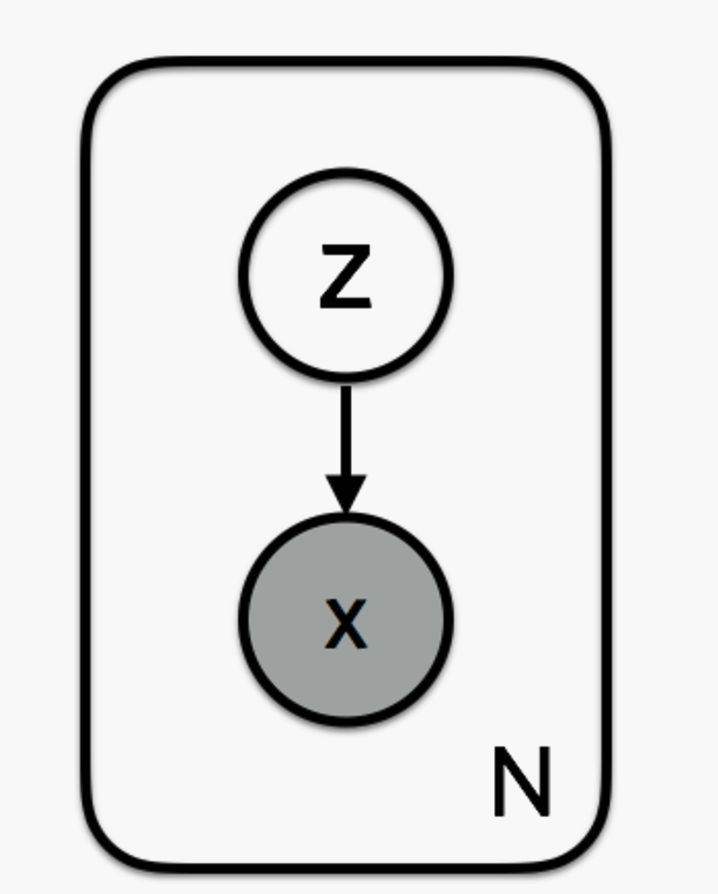
\includegraphics[width=4cm, height=5cm]{vae.png}
\end{center}
\subsubsection{Inference}

The goal is to infer good values of the latent variables given observed data, or to calculate the posterior p(z|x).

$p(z|x) = \frac{p(x|z)p(z)}{p(x)}$

Examine the denominator p(x). This is evidence, we can calculate it by marginalizing out the latent variables:
$p(x) = \int p(x|z)p(z)dz$. This integral requires exponential time to compute as it needs to be evaluated over all configurations of latent variables. So we need to approximate this posterior distribution.

Variational inference approximates the posterior with a family of distributions $q_\lambda(z|x)$. This lambda indexes the family of distributions. If q were Gaussian, it would be the mean and variance of the latent variables for each datapoint $\lambda_{x_i}=(\mu_{x_i},\sigma^2_{x_i})$

How well our $q(z|x)$ approximates the true $p(z|x)$? We use KL divergence, 

$KL(q_\lambda||p) = E_q[log q_\lambda(z|x)] - E_q[log p(x,z)] + log p(x)$ 

Object: 
$q^*_\lambda(z|x) = arg min_\lambda KL(q_\lambda(z|x)||p(z|x))$

However, p(x) appears in the divergence. This is intractable. We need one more ingredient for tractable variational inference. 

$ELBO(\lambda) = E_q[log p(x,z)] - E_q[log q_\lambda(z|x)]$

So we have

$log p(x) = ELBO(\lambda) + KL(q_\lambda(z|x)||p(z|x))$

$KL >= 0 $, by Jensen's inequality. So minimizing the KL divergence is equivalent to maximizing the ELBO. p(x) is fixed.

{\bf ELBO = Evidence Lower BOund} allows us to do approximate posterior inference. So instead of computing and minimizing the KL divergence, we can maximize the ELBO

$ELBO_i(\lambda) = E_{q\lambda}[logp(x_i|z)] - KL(q_\lambda(z|x_i)||p(z))$

$ELBO(\lambda) = E_q[logp(x,z)] - E_q[logq_\lambda(z|x)] = 
E_q[log p(x|z)p(z)] - E_q[logq_\lambda(z|x)] = E_q[log p(x|z)] + E_q[log p(z)] - E_q[logq_\lambda(z|x)] = E_{q\lambda}[logp(x_i|z)] - KL(q_\lambda(z|x_i)||p(z))$. Here the E[ ] gives the p(z)

Let’s make the connection to neural net language. The final step is to parametrize the approximate posterior $q_\theta (z | x, \lambda)$
 with an inference network (or encoder) that takes as input data xx and outputs parameters $\lambda$. We parametrize the likelihood $p(x |z)$ with a generative network (or decoder) that takes latent variables and outputs parameters to the data distribution $p_\phi(x|z)$. The inference and generative networks have parameters $\theta$ and $\phi$ respectively. The parameters are typically the weights and biases of the neural nets. We optimize these to maximize the ELBO using stochastic gradient descent.
 
 So ELBO this evidence lower bound is the negative of the loss function for variational autoencoders.

\subsection{Connectionist Temporal Classification (CTC)}

For a given X it gives us an output distribution over all possible Y's. We can use this distribution either to infer a likely output or to assess the probability of a given output.

{\bf Loss Function}: Compute p(Y|X)

{\bf Inference}: Solving $Y* = argmax_Y p(Y|X)$

CTC algorithm is alignment-free, it doesn't require an alignment bweetn input and the output. 

CTC introduces a new token: blank token. 

\begin{center}
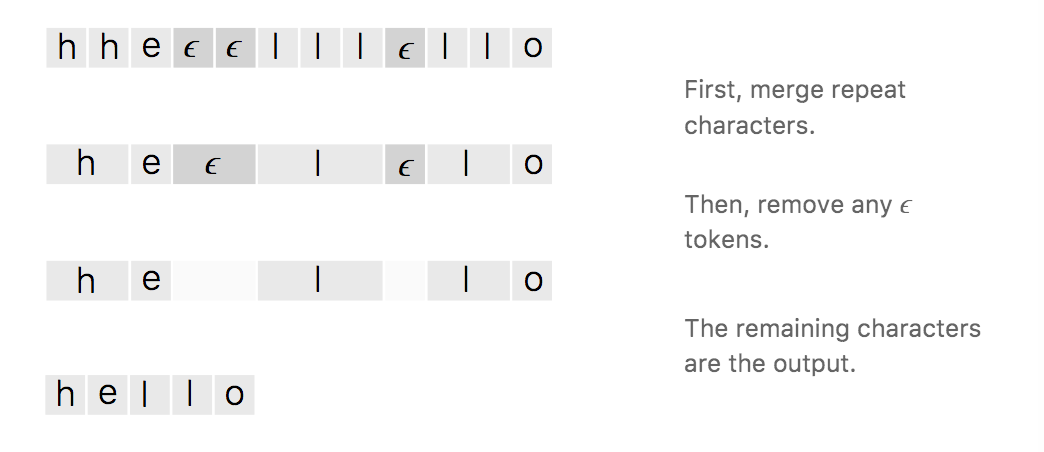
\includegraphics[width=8cm, height=4cm]{blank.png}
\end{center}

The CTC alginments give us a natural way to go from probabilities at each time-step to the probability of an output sequence.

\begin{center}
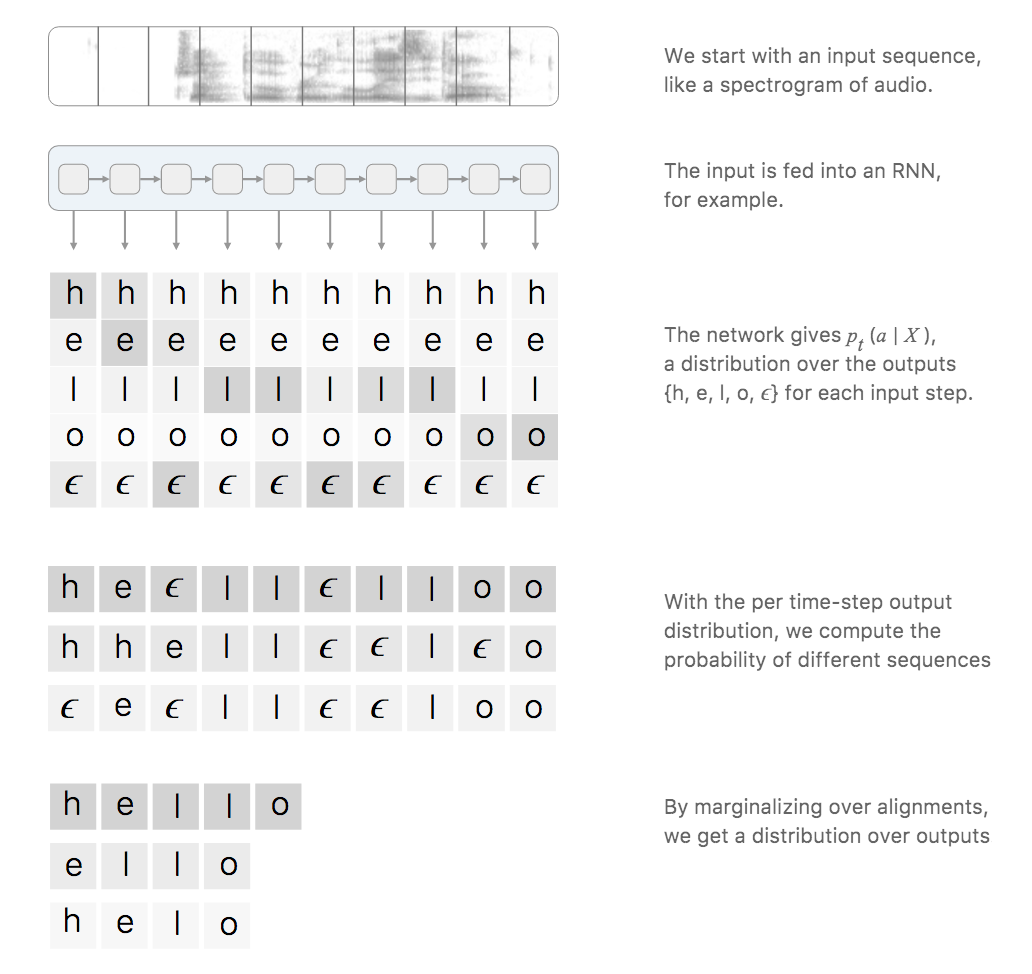
\includegraphics[width=6cm, height=6cm]{ctc.png}
\end{center}

The CTC object for a single (X, Y) pair is:

$ p(Y|X) = \sum_{A in A_{X,Y}} \prod_{t=1}^T p_t(a_t|X)$

The CTC conditional probability; marginalizes over the set of valid alignments; computing the probability for a single alignment step-by-step.

$p_t(a_t|X)$ is trained by using a recurrent neural network. 

We can compute the loss much faster with a dynamic programming algorithm. Key: if two alignments have reached the same output at the same step, then we can merge them.

<img src="dp.png" alt="Drawing" style="width: 300px;"/>
Let $\alpha$ be the score of the merged alignments at a given node. If $\alpha_{s,t}$ is the CTC score of the subsequence $Z_{1:s}$ after t input steps. We will compute CTC score P(Y|X) from the $\alpha$'s at the last time-step.

$Z = [\epsilon,y_1,\epsilon,y_2,...,\epsilon,y_U,\epsilon]$

\subsubsection{Case 1}
$\alpha_{s,t} = (\alpha_{s-1,t-1}+\alpha_{s,t-1})*p_t(z_s|X)$

two cases: 1 is from blank to a, 1 is from a to a again(repeat).

\subsubsection{Case 2}

$\alpha_{s,t} = (\alpha_{s-1,t-1}+\alpha_{s,t-1})*p_t(z_s|X)$

two cases: 1 is from blank to a, 1 is from a to a again(repeat).

\subsubsection{Case 2}

when $z_{s-1}$ is $\epsilon$, we have 3 cases:

1. a

2. $\epsilon$

3. b

so 

$\alpha_{s,t} = (\alpha_{s-2,t-1}+\alpha_{s-1,t-1}+\alpha_{s,t-1})p_t(z_s|X)$

\begin{center}
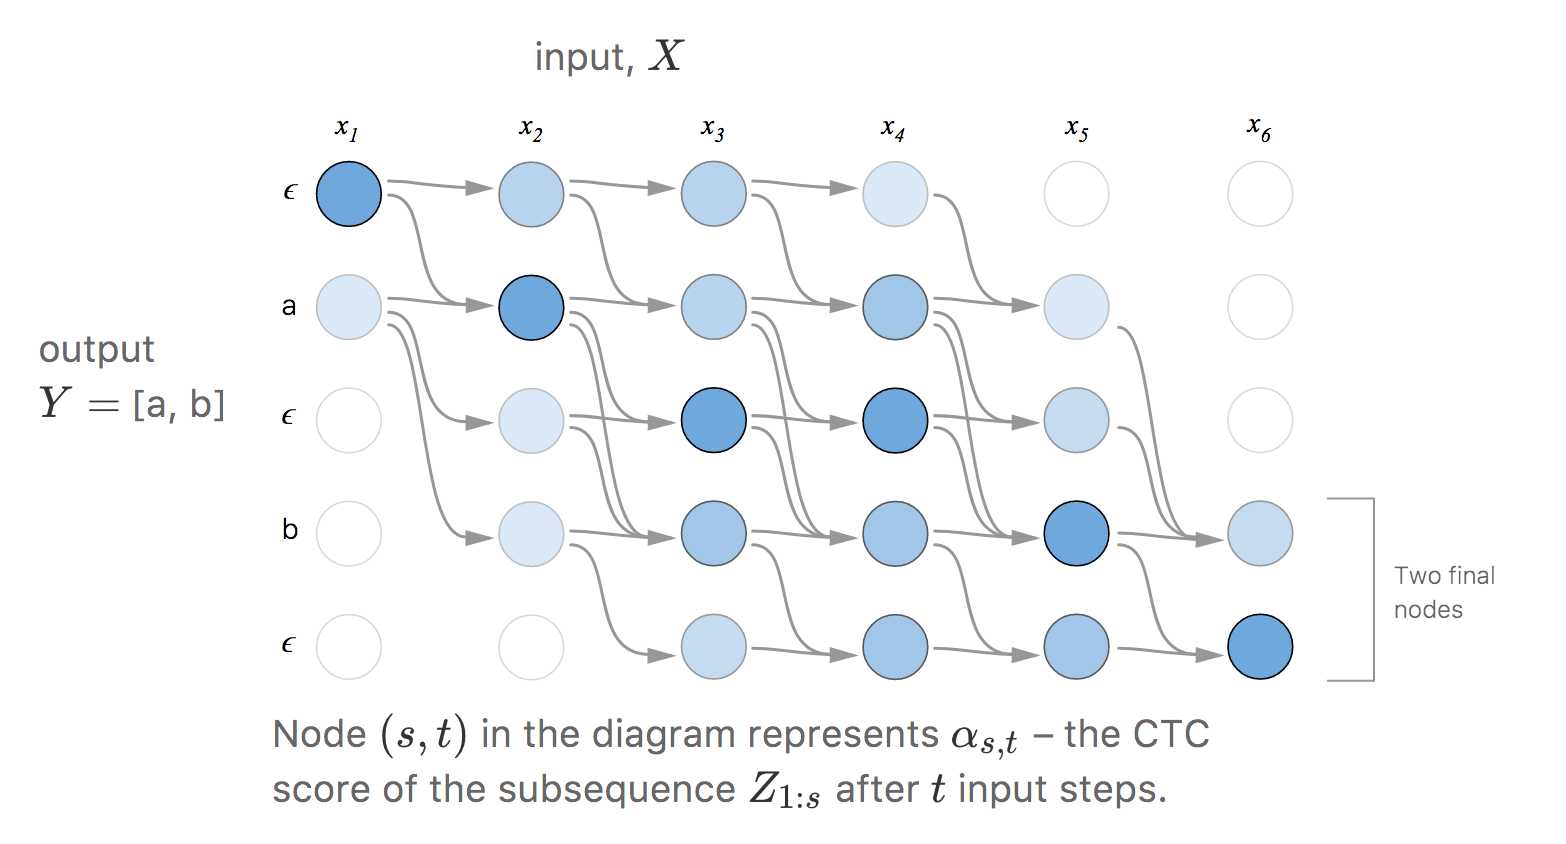
\includegraphics[width=10cm, height=6cm]{dp_g.png}
\end{center}
%<img src="dp_g.png" alt="Drawing" style="width: 300px;"/>

There are two valid starting nodes and two valide final nodes since the $\epsilon$ at the begining and end of the sequence is optional. The complete probability is the sum of the two final nodes.

So the object is to minimize the negative log-likelihood
$\sum_{(X,Y) in D} - log p(Y|X)$

\subsubsection{Inference}

We need to solve:

$Y^* = argmax_Y p(Y|X)$

$A* = argmax_A \prod_{t=1}^T p_t(a_t|X)$

use modifed beam search:
we can modify the vanilla beam search to handle multiple alignments mapping to the same output. In this case instead of keeping a list of alignments in the beam, we store the output prefixes after collapsing repeats and removing $\epsilon$ characters. At each step of the search we accumulate scores for a given prefix based on all alignments which map to it.

\begin{center}
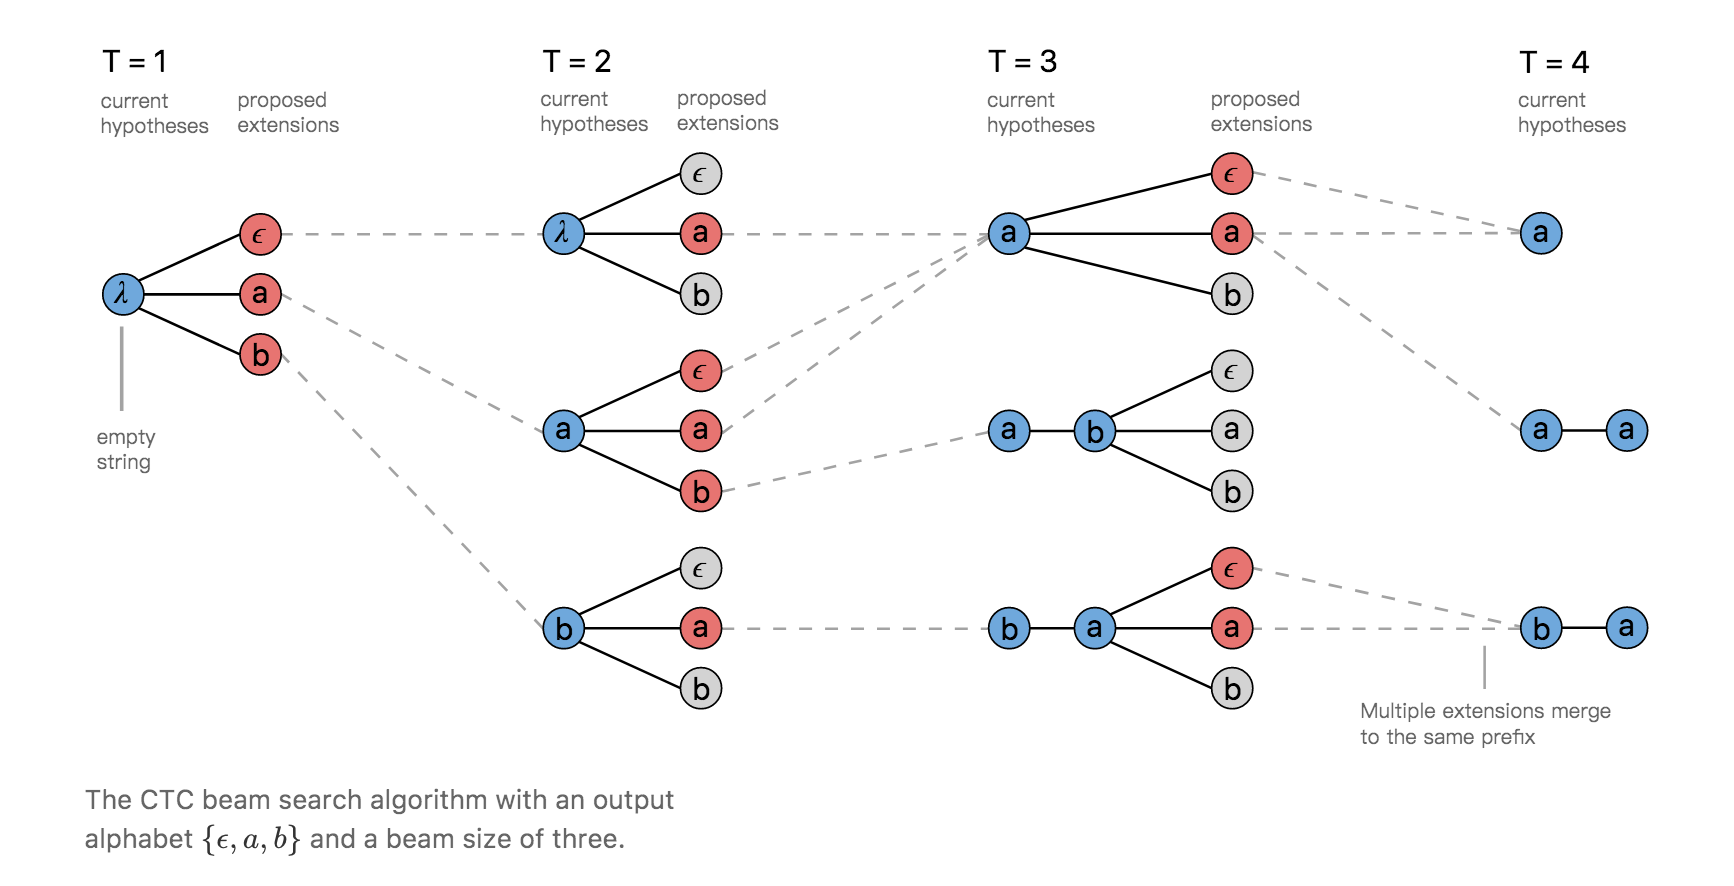
\includegraphics[width=10cm, height=6cm]{bs.png}
\end{center}

$Y^*= argmax_Y p(Y|X)p(Y)^{\alpha}L(Y)^{\beta}$

p(Y) is the language model probability. L(Y) computes the lenght of Y in terms of the language model tokens and acts as a word insertion bonous.

% -----------------------------------------------
% Ignore everything that appears below this.
% -----------------------------------------------
\end{document}
